%XeLaTex+MakeIndex+BibTex%
\documentclass[12pt]{article}
\usepackage{fontspec}
\usepackage{polyglossia}
\usepackage{geometry}
\usepackage{xcolor}
\usepackage{titlesec}
\usepackage{fancyhdr}
\usepackage{graphicx}
\usepackage{mathtools}
\graphicspath{{../matlab/figures/}}
\usepackage{hyperref} % Add hyperref package for clickable links
\usepackage{amsmath}
\usepackage{tabularx}

\usepackage{float}
\usepackage{caption}
\usepackage{subcaption}

% Set the page margins
\geometry{a4paper,margin=2.54cm}

\usepackage{kmath,kerkis} % The order of the packages matters; kmath changes the default text font
%\usepackage[T1]{fontenc}

% Set the font to Kerkis
\setmainfont{Kerkis}


\usepackage{matlab-prettifier}

% Define colors
\definecolor{myblue}{RGB}{0, 51, 102}
\definecolor{mygray}{RGB}{150,150,150}
\definecolor{mybg}{RGB}{230,230,230}

% Set line spacing
\usepackage{setspace}  % Required for custom line spacing
\setstretch{1.15}      % Set custom line spacing

% Set section title formatting
\titleformat{\section}
  {\normalfont\Large\bfseries\color{myblue}}
  {\thesection}{1em}{}
%\titleformat{\subsection}
%  {\normalfont\Large\bfseries\color{myblue}}
%  {\thesubsection}{1em}{}

\setmainlanguage{english}

% Define header and footer
\pagestyle{fancy}
\fancyhf{}
\lhead{Team 2}
\rhead{Evolutionary Games Toolbox}
\rfoot{\thepage}


\begin{document}
\begin{titlepage}
\newgeometry{margin=2.54cm, tmargin=3cm, bmargin=3cm}
\centering
\begin{figure}[H]
\centering
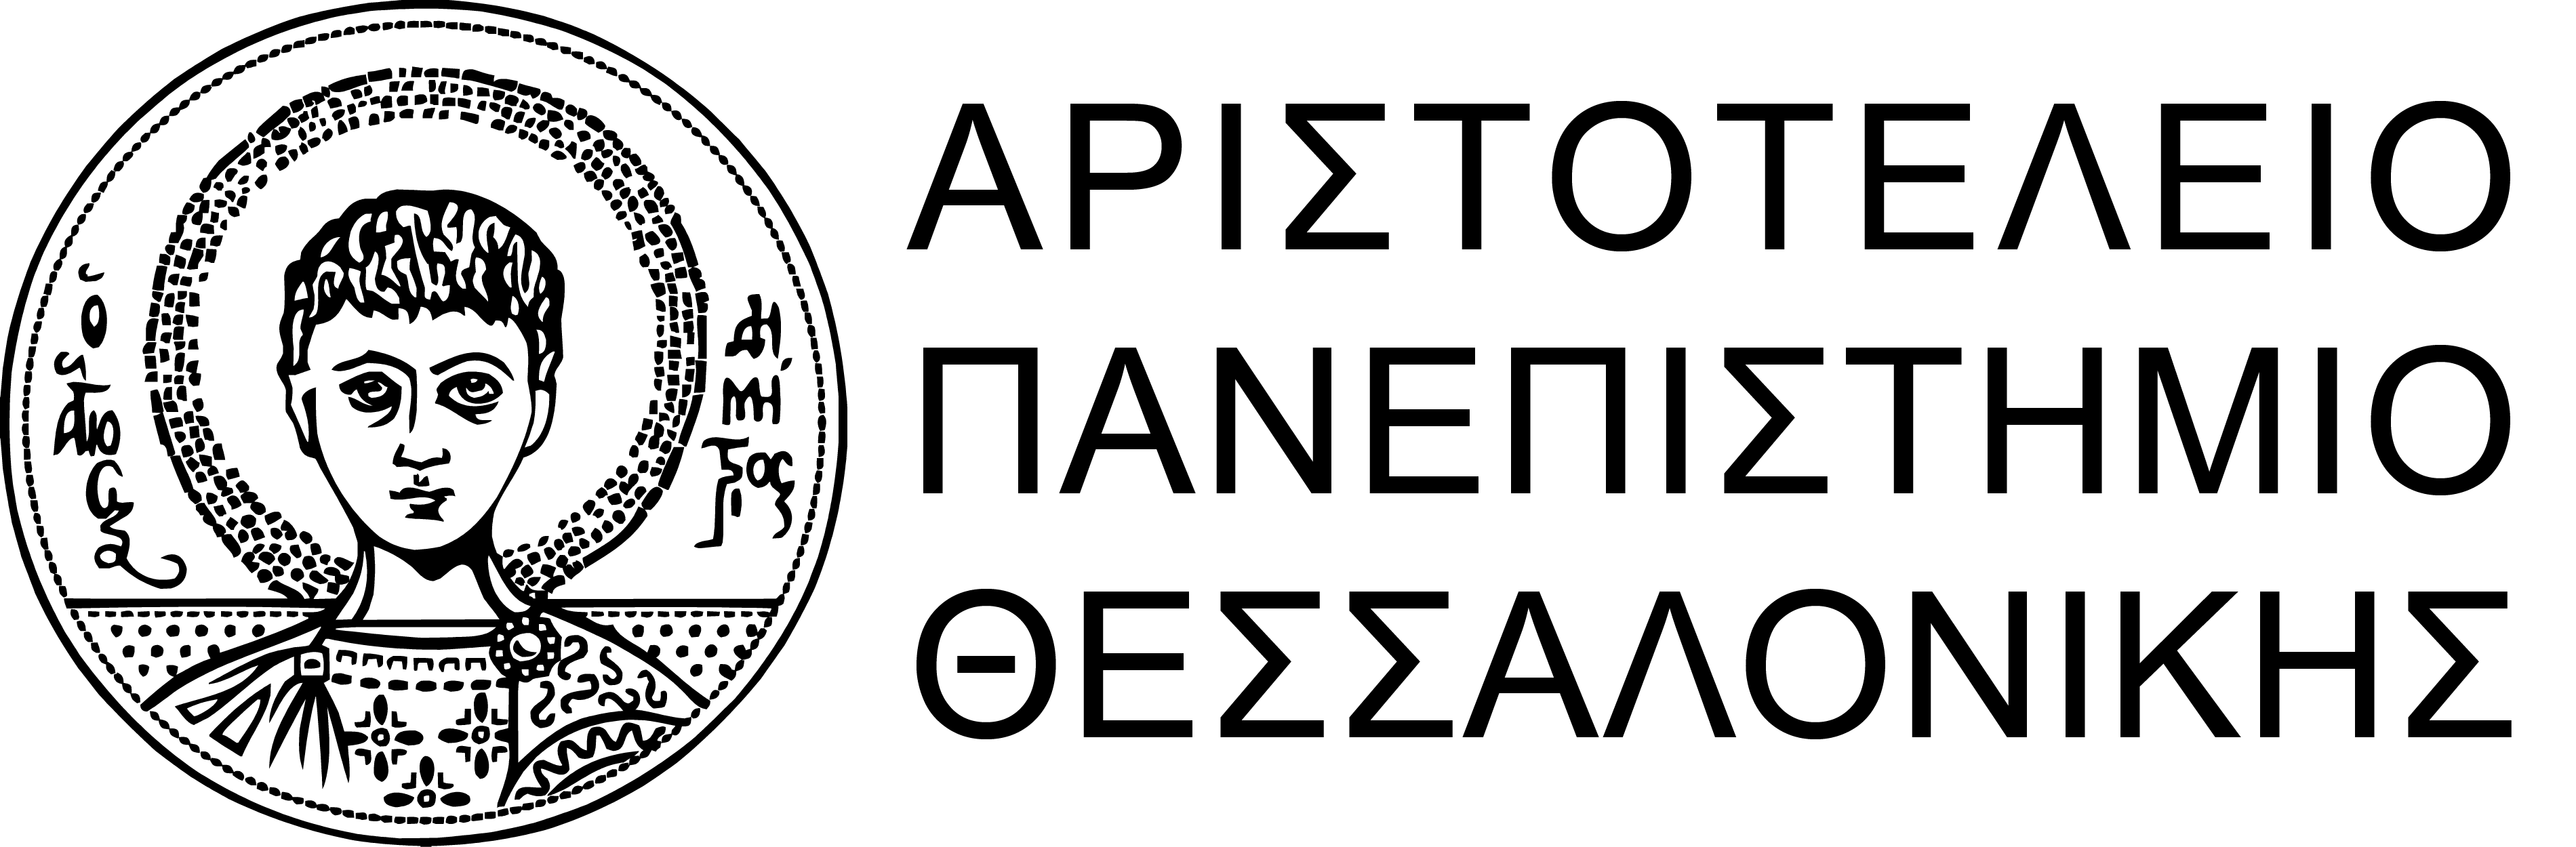
\includegraphics[width=0.8\textwidth]{banner-horizontal-black300ppi.png}\par % Image on top of title
\end{figure}
%\textcolor{black}{\large \bfseries Αριστοτέλειο Πανεπιστήμιο Θεσσαλονίκης\\}\par
\vspace{18pt}
\textcolor{black}{\Large \bfseries Department of Electrical\\and Computer Engineering\\}\par
\vspace{1cm}
\vfill
\textcolor{black}{\Large \bfseries Game Theory}\par
\vspace{12pt}
\textcolor{black}{\large \bfseries Evolutionary Games Toolbox - Documentation}\par

\vspace{0.5cm} % Adjust vertical spacing here
\vfill
\newcolumntype{L}{>{\raggedright\arraybackslash}X}%
\newcolumntype{R}{>{\raggedleft\arraybackslash}X}%
{\large
\def\arraystretch{1.3}
\begin{tabularx}{\textwidth}{ R|L }
\textbf{Team}                			 & 2           \\
\textbf{Vaporis Dimitrios}      & ΑΕΜ 10625 \\
\textbf{Voulkidis Vlasios}        & ΑΕΜ 10627 \\
\textbf{Delopoulos Emmanouil}      & ΑΕΜ 10693 \\
\textbf{Professor}           & Kehagias Athanasios\\
\end{tabularx}
}
\vspace{0.5cm}
\vfill
\textcolor{black}{\large \bfseries Spring Semester 2025}\par
\end{titlepage}
\restoregeometry

\tableofcontents % Table of Contents

\clearpage
\section{Introduction}
The following is a file containing the documentation for the Evolutionary Games Toolbox contained in this GitHub repository. It is split into three segments: in the first segment, the documentation of each function contained in the Code folder are presented, whereas in the second segment, the simulation correspoding to each example file in the Examples folder is noted. Lastly, the third segment contains documentation on the strategies in the strategies subfolder of the Code folder. Note that the details regarding the operation of each function are not presented in this file (a lot of this is done in the Report.pdf file in the Report folder). Instead, this is a showcase of what each function expects as input, what it returns as output, which example corresponds to which simulation and how each strategy of the toolbox behaves. Across the functions written, there are smaller helper functions that are not included in this documentation, for the sake of simplicity.

\section{Functions of Code folder}
This is the documentation of the functions contained in the Code folder. The inputs/outputs of each functions are presented, without showcasing the operation of each one. See also the Report.pdf as well as the source code of each function (it is properly commented) if necessary.

\subsection{AnalyzeMarkovChain}
The AnalyzeMarkovChain function is responsible for creating the directed state graphs of the Imitation Dynamics. It requires inputs $P$ the transition matrix of the Markov Chain (usually calculated by the TourTheImi function), $POP0$ the initial $1 \times S$ (with $S$ the number of strategies used in the simulation) population vector, $Strategies$ an array containing the string names of the strategies used in the simulation (as named later on in the Strategies section) and $Title$ the string containing the title of the outgoing graph. The function does not have any outputs, as it only creates the graph and exports it for use in the Report).

\subsection{Axel}
The Axel function computes the score of a single generation Axelrod tournament between specific strategies. It expects inputs $B$ a $2 \times 2$ payoff matrix for each match, $Strategies$ an array containing the string names of the strategies used in the simulation (as named later on in the Strategies section), $Pop$ the initial $1 \times S$ (with $S$ the number of strategies used in the simulation) population vector and $T$ the number of rounds played in each match of the tournament. It returns an $N \times 1$ array (with $N$ being the total number of players in the simulation) containing the score of each player of the simulation at the end of the Axelrod tournament. Note that this function is not used for functions later on because of other faster implementations used.

\subsection{plotFitnessVSImitation}
The plotFitnessVSImitation function creates and exports a figure comparing the Fitness and Imitation Dynamics, using both ``Total'' and ``Individual'' mode for best strategy calculation in the Imitation Dynamics. It expects inputs $Strategies$ an array containing the string names of the strategies used in the simulation (as named later on in the Strategies section), $POP1$ the population matrix for each generation of the Fitness Dynamics (created by TourSimFit), $POP2$ the population matrix for each generation of the Imitation Dynamics - ``Individual'' mode (created by TourSimImi), $POP3$ the population matrix for each generation of the Imitation Dynamics - ``Total'' mode (created by TourSimImi with ``Total'' mode input) and $Title$ the title string of the created graph. The function does not have outputs and only creates and exports the graph. See example10 for an example usage of the function.

\subsection{plotPopulationOfStrategiesOverGenerations}
The plotPopulationOfStrategiesOverGenerations function constructs the diagram of populations of different strategies across generations after a completed simulation. It requires inputs $Strategies$ an array containing the string names of the strategies used in the simulation (as named later on in the Strategies section), $POP$ the population matrix for each generation of the given simulation, created by the corresponding function and $Title$ the title string of the created diagram. The function does not have outputs and only creates and exports the diagram graphing the population of each strategy with respect to the generation number.

\subsection{plotPopulationsOfStrategiesOverGenerations}
The plotPopulationsOfStrategiesOverGenerations function creates the plots for the population of different strategies across generations for results generated by TourTheFit, TourSimFit with compensation and without compensation. It expects inputs $Strategies$ an array containing the string names of the strategies used in the simulation (as named later on in the Strategies section), $POP1$ the theoretical population matrix for each generation of the Fitness Dynamics (created by TourTheFit), $POP2$ the population matrix for each generation of the Fitness Dynamics without compensation (created by TourSimFit), $POP3$ the population matrix for each generation of the Fitness Dynamics with compensation (created by TourSimFit with $compensation$ = true input) and $Title$ the title string of the created figure. The function does not have outputs and only creates and exports the figure. See the first few examples for example usages of the function.

\subsection{plotPopulationsTourSimImi}
The plotPopulationsTourSimImi function creates the plot for the population of different strategies across generations after a completed TourSimImi simulation. It expects inputs $Strategies$ an array containing the string names of the strategies used in the simulation (as named later on in the Strategies section), $POP$ the population matrix for each generation of the given simulation, created by the TourSimImi function and $Title$ the title string of the created plot. The function does not have outputs and only creates and exports the diagram graphing the population of each strategy with respect to the generation number. See example07 for an example usage of the function.

\subsection{TourSimFit}
The TourSimFit function simulates the evolutionary tournament using Fitness Dynamics. The function expects inputs $B$ a $2 \times 2$ payoff matrix for each match, $Strategies$ an array containing the string names of the strategies used in the simulation (as named later on in the Strategies section), $POP0$ the initial $1 \times S$ (with $S$ the number of strategies used in the simulation) population vector, $T$ the number of rounds played in each match of the tournament, $J$ the number of generations of the simulation and $compensation$ an optional argument (with default value being false) that toggles the usage of random compensation to keep the total population of each generation constant (this is better explained in the Report). It returns a $(J+1) \times S$ array $POP$ containing the population of each generation for each strategy, a $J \times S$ array $BST$ containing information about the best strategy of each generation (for the cell $(i,j)$ of the array, if it has value 1 then strategy $j$ was the best for generation $i$, else it has value 0) and $FIT$ a $J \times S$ array that contains the fitness scores of each strategy for each generation.

\subsection{TourSimImi}
The TourSimImi function simulates the evolutionary tournament using Imitation Dynamics. The function expects inputs $B$ a $2 \times 2$ payoff matrix for each match, $Strategies$ an array containing the string names of the strategies used in the simulation (as named later on in the Strategies section), $POP0$ the initial $1 \times S$ (with $S$ the number of strategies used in the simulation) population vector, $T$ the number of rounds played in each match of the tournament, $J$ the number of generations of the simulation and $mode$ an optional argument (with default value being ``Individual'') that toggles the mode for best strategy selection, with the other option being ``Total'' (this is better explained in the Report). It returns a $(J+1) \times S$ array $POP$ containing the population of each generation for each strategy and a $J \times S$ array $BST$ containing information about the best strategy of each generation (for the cell $(i,j)$ of the array, if it has value 1 then strategy $j$ was the best for generation $i$, else it has value 0).

\subsection{TourTheFit}
The TourTheFit function conducts the theoretical analysis of an evolutionary tournament using Fitness Dynamics. The function expects inputs $B$ a $2 \times 2$ payoff matrix for each match, $Strategies$ an array containing the string names of the strategies used in the simulation (as named later on in the Strategies section), $POP0$ the initial $1 \times S$ (with $S$ the number of strategies used in the simulation) population vector, $T$ the number of rounds played in each match of the tournament and $J$ the number of generations of the simulation. It returns a $(J+1) \times S$ array $POP$ containing the population of each generation for each strategy, a $J \times S$ array $BST$ containing information about the best strategy of each generation (for the cell $(i,j)$ of the array, if it has value 1 then strategy $j$ was the best for generation $i$, else it has value 0) and $FIT$ a $J \times S$ array that contains the fitness scores of each strategy for each generation.

\subsection{TourTheImi}
The function TourTheImi computes the state transition matrix of a given evolutionary tournament using Imitation Dynamics using Markov Chain theory. The function expects inputs $B$ a $2 \times 2$ payoff matrix for each match, $Strategies$ an array containing the string names of the strategies used in the simulation (as named later on in the Strategies section), $POP0$ the initial $1 \times S$ (with $S$ the number of strategies used in the simulation) population vector, $T$ the number of rounds played in each match of the tournament, $J$ the number of generations of the simulation and $mode$ an optional argument (with default value being ``Individual'') that toggles the mode for best strategy selection, with the other option being ``Total'' (this is better explained in the Report). It returns an array $P$ which is the state transition matrix of the process. More specifically, the cell $(i,j)$ of the array contains the probability that the system reaches state $j$ at the next step, given that the system starts at state $i$ (with system being the population distribution and each state being each possible population distribution). Use AnalyzeMarkovChain to visualize and understand the results.

\section{Examples of Examples folder}
This is the documentation of the Examples contained in the Examples folder of the repository. More specifically, the situation each example simulates is presented and any possible links to the paper by Mathieu et al are mentioned.

\subsection{example01}
The first example shows the results of TourTheFit, TourSimFit with compensation and TourSimFit without compensation in the case presented by Mathieu et al in Figure 1, with Title ``Defectors may be strong''. The functions are called with payoff matrix $B = \begin{bmatrix} 3 & 0 \\ 5 & 1 \end{bmatrix}$, $Strategies = ["per\_ddc", "Alternator", "soft\_majo"]$, initial population $POP0 = [100; 100; 100]$, number of rounds per match $T = 1000$ and number of generations $J = 90$.

\subsection{example02}
This shows the results of TourTheFit, TourSimFit with compensation and TourSimFit without compensation in the case presented by Mathieu et al in Figure 2, with Title ``Monotonous convergence''. The functions are called with payoff matrix $B = \begin{bmatrix} 3 & 0 \\ 5 & 1 \end{bmatrix}$, $Strategies = ["Grim", "TitForTat", "Alternator"]$, initial population $POP0 = [100; 100; 100]$, number of rounds per match $T = 1000$ and number of generations $J = 10$.

\subsection{example03}
This shows the results of TourTheFit, TourSimFit with compensation and TourSimFit without compensation in the case presented by Mathieu et al in Figure 3, with Title ``Attenuated oscillatory movements''. The functions are called with payoff matrix $B = \begin{bmatrix} 3 & 0 \\ 5 & 1 \end{bmatrix}$, $Strategies = ["per\_ccd", "per\_ddc", "soft\_majo"]$, initial population $POP0 = [450; 1000; 100]$, number of rounds per match $T = 1000$ and number of generations $J = 420$.

\subsection{example04}
This shows the results of TourTheFit, TourSimFit with compensation and TourSimFit without compensation in the case presented by Mathieu et al in Figure 4, with Title ``Periodic movements''. The functions are called with payoff matrix $B = \begin{bmatrix} 3 & 0 \\ 5 & 1 \end{bmatrix}$, $Strategies = ["per\_ccd", "per\_ddc", "soft\_majo"]$, initial population $POP0 = [300; 200; 100]$, number of rounds per match $T = 1000$ and number of generations $J = 1000$.

\subsection{example05}
This shows the results of TourTheFit, TourSimFit with compensation and TourSimFit without compensation in the case presented by Mathieu et al in Figure 5, with Title ``Increasing oscillations''. The functions are called with payoff matrix $B = \begin{bmatrix} 3 & 0 \\ 4.72 & 1 \end{bmatrix}$, $Strategies = ["per\_ccd", "per\_ddc", "soft\_majo"]$, initial population $POP0 = [300; 400; 200]$, number of rounds per match $T = 1000$ and number of generations $J = 450$.

\subsection{example06}
This shows the results of TourTheFit, TourSimFit with compensation and TourSimFit without compensation in the case presented by Mathieu et al in Figure 6, with Title ``Disordered oscillations''. The functions are called with payoff matrix $B = \begin{bmatrix} 3 & 0 \\ 5 & 1 \end{bmatrix}$, $Strategies = ["soft\_majo", "per\_ccccd", "Prober"]$, initial population $POP0 = [100; 500; 800]$, number of rounds per match $T = 1000$ and number of generations $J = 280$.

\subsection{example07}
This shows the results of TourTheFit, TourSimFit with compensation and TourSimFit without compensation in the case presented by Mathieu et al in the left plot of Figure 7, with Title ``Sensitivity of dynamics to population's size''. The functions are called with payoff matrix $B = \begin{bmatrix} 3 & 0 \\ 5 & 1 \end{bmatrix}$, $Strategies = ["per\_ccd", "soft\_majo", "per\_ddc"]$, initial population $POP0 = [300; 100; 244]$, number of rounds per match $T = 1000$ and number of generations $J = 1000$.

\subsection{example08}
This shows the results of TourTheFit, TourSimFit with compensation and TourSimFit without compensation in the case presented by Mathieu et al in the right plot of Figure 7, with Title ``Sensitivity of dynamics to population's size''. The functions are called with payoff matrix $B = \begin{bmatrix} 3 & 0 \\ 5 & 1 \end{bmatrix}$, $Strategies = ["per\_ccd", "soft\_majo", "per\_ddc"]$, initial population $POP0 = [300; 100; 245]$, number of rounds per match $T = 1000$ and number of generations $J = 1000$.

\subsection{example09}
This shows the results of TourTheFit, TourSimFit with compensation and TourSimFit without compensation in the case presented by Mathieu et al in the left plot of Figure 8, with Title ``Sensitivity of winner to population's size''. The functions are called with payoff matrix $B = \begin{bmatrix} 3 & 0 \\ 5 & 1 \end{bmatrix}$, $Strategies = ["per\_ddc", \- "soft\_majo", \-"Alternator"]$, initial population $POP0 = [100; 159; 100]$, number of rounds per match $T = 1000$ and number of generations $J = 120$.

\subsection{example10}
This shows the results of TourTheFit, TourSimFit with compensation and TourSimFit without compensation in the case presented by Mathieu et al in the right plot of Figure 8, with Title ``Sensitivity of winner to population's size''. The functions are called with payoff matrix $B = \begin{bmatrix} 3 & 0 \\ 5 & 1 \end{bmatrix}$, $Strategies = ["per\_ddc", "soft\_majo", "Alternator"]$, initial population $POP0 = [100; 160; 100]$, number of rounds per match $T = 1000$ and number of generations $J = 120$.

\subsection{example11}
This shows the results of TourTheFit, TourSimFit with compensation and TourSimFit without compensation in the case presented by Mathieu et al in the left plot of Figure 9, with Title ``Sensitivity to game length''. The functions are called with payoff matrix $B = \begin{bmatrix} 3 & 0 \\ 5 & 1 \end{bmatrix}$, $Strategies = ["per\_ccd", "soft\_majo", "per\_ddc"]$, initial population $POP0 = [300; 100; 244]$, number of rounds per match $T = 7$ and number of generations $J = 1000$.

\subsection{example12}
This shows the results of TourTheFit, TourSimFit with compensation and TourSimFit without compensation in the case presented by Mathieu et al in the right plot of Figure 9, with Title ``Sensitivity to game length''. The functions are called with payoff matrix $B = \begin{bmatrix} 3 & 0 \\ 5 & 1 \end{bmatrix}$, $Strategies = ["per\_ccd", "soft\_majo", "per\_ddc"]$, initial population $POP0 = [300; 100; 244]$, number of rounds per match $T = 6$ and number of generations $J = 1000$.

\subsection{example13}
This shows the results of TourTheFit, TourSimFit with compensation and TourSimFit without compensation in the case presented by Mathieu et al in the left plot of Figure 10, with Title ``Sensitivity to CIPD payoff''. The functions are called with payoff matrix $B = \begin{bmatrix} 3 & 0 \\ 4.6 & 1 \end{bmatrix}$, $Strategies = ["per\_ccd", "soft\_majo", "per\_ddc"]$, initial population $POP0 = [300; 100; 244]$, number of rounds per match $T = 1000$ and number of generations $J = 1000$.

\subsection{example14}
This shows the results of TourTheFit, TourSimFit with compensation and TourSimFit without compensation in the case presented by Mathieu et al in the right plot of Figure 10, with Title ``Sensitivity to CIPD payoff''. The functions are called with payoff matrix $B = \begin{bmatrix} 3 & 0 \\ 4.7 & 1 \end{bmatrix}$, $Strategies = ["per\_ccd", "soft\_majo", "per\_ddc"]$, initial population $POP0 = [300; 100; 244]$, number of rounds per match $T = 1000$ and number of generations $J = 1000$.

\subsection{example15}
This shows the results of TourTheFit, TourSimFit with compensation and TourSimFit without compensation in the case presented by Mathieu et al in the plots of Figure 11, with Title ``Sensitivity to repartition computation method''. The functions are called with payoff matrix $B = \begin{bmatrix} 3 & 0 \\ 5 & 1 \end{bmatrix}$, $Strategies = ["per\_ccd", \- "soft\_majo", "per\_ddc"]$, initial population $POP0 = [300; 100; 200]$, number of rounds per match $T = 1000$ and number of generations $J = 1000$. Note that the plot on the left corresponds to the plot created by TourSimFit and the plot on the right corresponds to the one created by TourTheFit.

\subsection{example16}
This shows the results of TourTheFit, TourSimFit with compensation and TourSimFit without compensation in the case presented by Mathieu et al in the left plot of Figure 12, with Title ``Sensitivity to repartition computation method''. The functions are called with payoff matrix $B = \begin{bmatrix} 3 & 0 \\ 4.6 & 1 \end{bmatrix}$, $Strategies = ["per\_ccd", "soft\_majo", "per\_ddc"]$, initial population $POP0 = [450; 100; 1000]$, number of rounds per match $T = 1000$ and number of generations $J = 1000$.

\subsection{example17}
This shows the results of TourTheFit, TourSimFit with compensation and TourSimFit without compensation in the case presented by Mathieu et al in the right plot of Figure 12, with Title ``Sensitivity to repartition computation method''. The functions are called with payoff matrix $B = \begin{bmatrix} 3 & 0 \\ 4.6 & 1 \end{bmatrix}$, $Strategies = ["per\_ccd", "soft\_majo", "per\_ddc"]$, initial population $POP0 = [45; 10; 100]$, number of rounds per match $T = 1000$ and number of generations $J = 1000$.

\section{Strategies of strategies subfolder in the Code folder}
Lastly, this is the documentation for all strategies included in the strategies subfolder of the Code folder. For more details, the exact source code is available for each of the following strategies. Note that you can always enhance this collection with strategies of your own. For your created strategies to work with the toolbox, follow the format used in the strategies given: let the function have form function Move = YourStrategy(History), where History is the $T \times 2$ matrix of moves by both players for each turn, regard the player of your strategy as player 1 (the first column of the History matrix, it is flipped in case the player is actually player 2) and make Move = 2 in case of defection and Move = 1 in case of cooperation. Also, suppose that each strategy can only access past moves (player 2 cannot access player 1's current round move) and that each strategy does not know the amount of rounds played in each match. Lastly, because of the current form of simulation and theoretical analysis functions (that prioritize low running times), strategies including random elements are not included (in case you wish to include some, most functions will probably fail). For the strategies below, C stands for Cooperation and D stands for Defection.

\subsection{All\_C}
Strategy that always cooperates.

\subsection{All\_D}
Strategy that always defects.

\subsection{Alternator}
Strategy that alternates between cooperating and defecting, starting with cooperation in the first round.

\subsection{Cycler}
Strategy that permanently cycles the moves C, C, C, D.

\subsection{Detective}
Strategy that starts with the moves C, D, C, C. If the opponent defects at least once in these first four rounds, play as TitForTat forever. Else, always defect.

\subsection{Grim}
Strategy that always cooperates unless the opponent defects: after the first opponent defection, always defect.

\subsection{per\_ccccd}
Strategy that permanently cycles the moves C, C, C, C, D.

\subsection{per\_ccd}
Strategy that permanently cycles the moves C, C, D.

\subsection{per\_ddc}
Strategy that permanently cycles the moves D, D, C.

\subsection{Prober}
Strategy that starts with the moves D, C, C. If the opponent cooperates at moves 2 and 3, plays defect for the rest of the game. Otherwise plays as TitForTat.

\subsection{SneakyTitForTat}
Strategy that starts by cooperating in the first round and playing as TitForTat in the second round. If the opponent has not defected in these first two rounds, defect once and check the opponent's response. If the opponents retaliates, play a cooperation to repent and then play as TitForTat. If the opponent does not retaliate, keep playing defect and checking the opponent's response as before.

\subsection{soft\_majo}
Strategy that plays the same move as the majority of the opponent's moves up until the previous round. In case of equality, cooperate.

\subsection{SpitefulTitForTat}
Strategy that starts by cooperating and then plays like TitForTat, until the opponent defects twice in a row, in which case the player always defects.

\subsection{TitForTat}
Strategy that cooperates in the first move and for the rest of the game plays the opponent's previous move.

\subsection{TitForTwoTats}
Strategy that plays defect only if the opponent has defected twice in a row. Otherwise, always cooperates.

\subsection{TwoTitsForTat}
Strategy that starts by cooperating and replies to each opponent defection by two defections of its own. More specifically, if there has been a defection by the opponent in the two previous rounds, the player chooses defect. Otherwise, plays cooperate.

\end{document}